\documentclass[svgnames,11pt]{beamer}
\input{/home/tof/Documents/Cozy/latex-include/preambule_commun.tex}
\input{/home/tof/Documents/Cozy/latex-include/preambule_beamer.tex}
%\usepackage{pgfpages} \setbeameroption{show notes on second screen=left}
\author[]{Christophe Viroulaud}
\title{Algorithme glouton\\rendre la monnaie}
\date{\framebox{\textbf{Algo}}}
%\logo{}
\institute{Première - NSI}

\begin{document}
\begin{frame}
    \titlepage
\end{frame}
\begin{frame}
    \frametitle{}

    Il existe des machines automatiques qui peuvent rendre la monnaie.
    \begin{center}
        \centering
        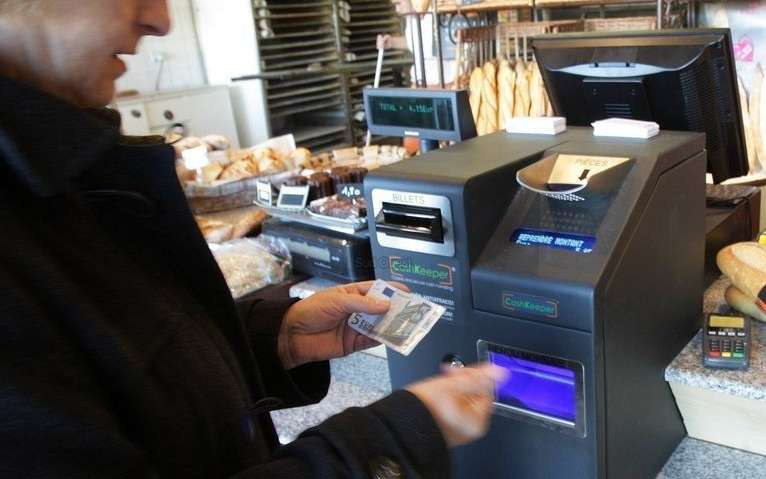
\includegraphics[width=8cm]{ressources/caisse.jpg}
        \captionof{figure}{\centering Caisse automatique dans une boulangerie}
        \label{IMG}
    \end{center}

\end{frame}
\begin{frame}
    \frametitle{}

    \begin{framed}
        \centering Quel algorithme mettre en place pour rendre la monnaie en utilisant le moins de pièces possibles?
    \end{framed}

\end{frame}
\begin{frame}
    \frametitle{}

    \begin{aretenir}[Remarques]
        \begin{itemize}
            \item Nous limiterons le problème aux valeurs entières.
            \item Nous n'utiliserons que les billets ou pièces de 1, 2, 5, 10€.
            \item On supposera que la caisse contient une quantité illimitée de monnaie.
        \end{itemize}
    \end{aretenir}

\end{frame}
\section{Approche exhaustive}
\begin{frame}
    \frametitle{Approche exhaustive}

    \begin{center}
        Il s'agit de tester toutes les combinaisons possibles avec les pièces dont nous disposons.

    \end{center}
\end{frame}
\begin{frame}
    \frametitle{Rendre 8€}

    \begin{center}
        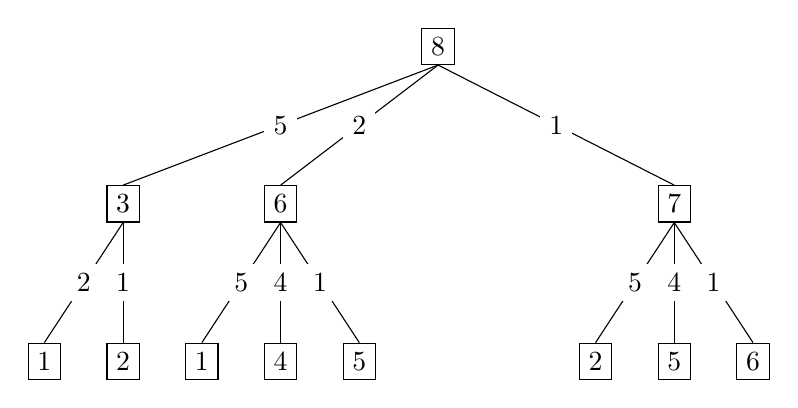
\begin{tikzpicture}
            \node[draw] (8-1) at(0,0){8};

            \node[draw] (3-2) at(-4,-2){3};
            \node[draw] (6-2) at(-2,-2){6};
            \node[draw] (7-2) at(3,-2){7};
            \draw (8-1.south) -- (3-2.north) node[midway, fill=white]{5};
            \draw (8-1.south) -- (6-2.north) node[midway, fill=white]{2};
            \draw (8-1.south) -- (7-2.north) node[midway, fill=white]{1};

            \node[draw] (1-4) at(-5,-4){1};
            \node[draw] (2-4) at(-4,-4){2};
            \draw (3-2.south) -- (1-4.north) node[midway, fill=white]{2};
            \draw (3-2.south) -- (2-4.north) node[midway, fill=white]{1};
            \node[draw] (1-42) at(-3,-4){1};
            \node[draw] (4-4) at(-2,-4){4};
            \node[draw] (5-4) at(-1,-4){5};
            \draw (6-2.south) -- (1-42.north) node[midway, fill=white]{5};
            \draw (6-2.south) -- (4-4.north) node[midway, fill=white]{4};
            \draw (6-2.south) -- (5-4.north) node[midway, fill=white]{1};

            \node[draw] (2-42) at(2,-4){2};
            \node[draw] (5-42) at(3,-4){5};
            \node[draw] (1-43) at(4,-4){6};
            \draw (7-2.south) -- (2-42.north) node[midway, fill=white]{5};
            \draw (7-2.south) -- (5-42.north) node[midway, fill=white]{4};
            \draw (7-2.south) -- (1-43.north) node[midway, fill=white]{1};
        \end{tikzpicture}
    \end{center}

\end{frame}
\begin{frame}
    \frametitle{}

    \begin{center}
        \centering
        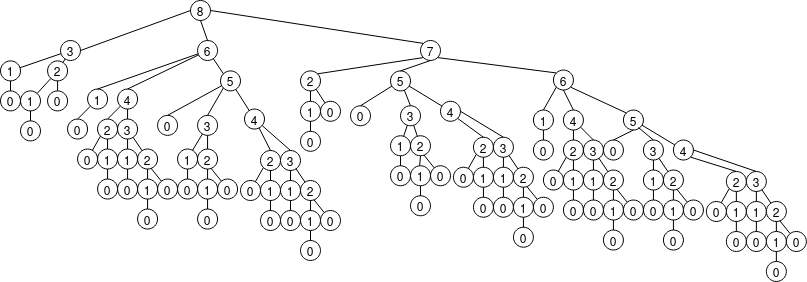
\includegraphics[width=10cm]{ressources/appel-naif-8.png}
        \captionof{figure}{Arbre des possibilités}
        \label{IMG}
    \end{center}

\end{frame}
\section{Approche gloutonne}
\subsection{Principe}
\begin{frame}
    \frametitle{Approche gloutonne - principe}
\begin{center}
    Pour éviter d'énumérer toutes les solutions possibles, on peut décider un seul choix à chaque étape et ne pas revenir dessus.
\end{center}
    

\end{frame}
\begin{frame}
    \frametitle{}

    \begin{aretenir}[]
        Un algorithme glouton construit un résultat global par une succession de choix intermédiaire donnant systématiquement le meilleur résultat partiel.
    \end{aretenir}

\end{frame}
\begin{frame}
    \frametitle{}

    \begin{center}
        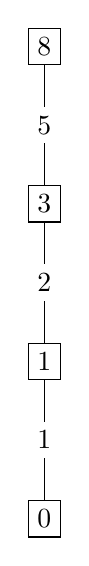
\begin{tikzpicture}
            \node[draw] (8) at(0,6){8};
            \node[draw] (3) at(0,4){3};
            \node[draw] (1) at(0,2){1};
            \node[draw] (0) at(0,0){0};
            \draw (8) -- (3) node[midway, fill=white]{5};
            \draw (3) -- (1) node[midway, fill=white]{2};
            \draw (1) -- (0) node[midway, fill=white]{1};
        \end{tikzpicture}
        \captionof{figure}{\centering On rend la plus grande pièce possible.}
    \end{center}

\end{frame}
\subsection{Propriétés}
\begin{frame}
    \frametitle{Propriétés}
Une approche gloutonne est:
    \begin{itemize}
        \item<1-> plus rapide qu'une solution exhaustive,
        \item<2-> plus simple à implémenter,
        \item<3-> \textbf{ne donne pas forcément la meilleure solution}
    \end{itemize}

\end{frame}
\begin{frame}
    \frametitle{}

L'ancien système britannique est composé de pièces: 1, 3, 4.\\
Pour rendre 6, l'algorithme glouton propose: 4, 1, 1.\\Alors qu'une autre solution optimale existe: 3, 3

\end{frame}
\subsection{Implémentation}
\begin{frame}[fragile]
    \frametitle{Implémentation}

\begin{center}
\begin{lstlisting}[language=Python , basicstyle=\ttfamily\small, xleftmargin=2em, xrightmargin=2em]
systeme = [10, 5, 2, 1]
\end{lstlisting}
\captionof{code}{On représente le système monétaire par un tableau.}
\label{CODE}
\end{center}
\begin{activite}
Écrire la fonction \textbf{\texttt{rendu(somme: int, systeme: list) $\rightarrow$ list}} qui renvoie le tableau des pièces à choisir pour rendre \textbf{\texttt{somme}}. La fonction implémentera l'algorithme suivant:\\
Tant que la somme à rendre n'est pas nulle:
\begin{itemize}
    \item sélectionner la plus grande pièce possible,
    \item la stocker dans un tableau,
    \item la soustraire à la somme à rendre.
\end{itemize}
\end{activite}
\end{frame}
\begin{frame}[fragile]
    \frametitle{Correction}

\begin{center}
\begin{lstlisting}[language=Python , basicstyle=\ttfamily\small, xleftmargin=.5em, xrightmargin=-1em]
def rendu_monnaie(somme: int, systeme: list) -> list:
    res = []
    while somme != 0:
        # choisir la pièce la plus grande possible
        i_piece = 0
        while systeme[i_piece] > somme:
            i_piece += 1
        # stocker
        res.append(systeme[i_piece])
        # soustraire
        somme -= systeme[i_piece]
    return res

# appel de la fonction
rendu_monnaie(14, [10, 5, 2, 1])
\end{lstlisting}
\captionof{code}{possibilité 1}
\label{CODE}
\end{center}   

\end{frame}
\begin{frame}[fragile]
    \frametitle{Correction}

\begin{center}
\begin{lstlisting}[language=Python , basicstyle=\ttfamily\small, xleftmargin=.5em, xrightmargin=-1em]
def rendu_monnaie(somme: int, systeme: list) -> list:
    res = []
    i_piece = 0
    while somme > 0:
        # si pièce est trop grande
        if systeme[i_piece] > somme:
            # on avance dans le système
            i_piece += 1
        else:
            res.append(systeme[i_piece])
            somme -= systeme[i_piece]
    return res

# appel de la fonction
rendu_monnaie(14, [10, 5, 2, 1])
\end{lstlisting}
\captionof{code}{possibilité 2}
\end{center}    

\end{frame}
\end{document}